\documentclass[aip, jcp, reprint, twocolumn]{revtex4-2}

\bibliographystyle{apsrev4-2}

\usepackage{physics}
\usepackage{amsmath}
\usepackage{amssymb}
\usepackage{mathtools}
\usepackage{graphicx}
\usepackage{dcolumn}
\usepackage[colorlinks=true, linkcolor=black, urlcolor=blue, citecolor=black, anchorcolor=black]{hyperref}

\graphicspath{{"figures/"}}
\begin{document}
%Title of paper
\title{Coherent Hyper-Raman Four Wave Mixing Spectroscopies}

\author{Ryan P. McDonnell} 
\author{Daniel D. Kohler}
\author{John C. Wright} \email{wright@chem.wisc.edu}

\affiliation{Department of Chemistry, 
        University of Wisconsin - Madison, 
        Madison, Wisconsin 53706, 
        United States of America}

\date{\today}

\begin{abstract}
Nonlinear, four wave mixing vibrational spectroscopies are often used to probe intramolecular vibrational coupling and relaxation dynamics.
Three wave mixing vibrational spectroscopies are similarly often used to understand the spectroscopy and dynamics of interfacial species.
Most of these methods rely on infrared or Raman transitions to generate output. 
The implementation of a nonlinear hyper-Raman spectroscopy, which first appears at third order perturbation theory, can provide a useful analogue to these techniques.
Singly Vibrationally Enhanced (SIVE) spectroscopy, a type of nonlinear hyper-Raman spectroscopy, is an underdeveloped four wave mixing technique which shows promise to disentangle ultrafast vibrational dynamics in isotropic systems without need for anharmonicities.
We derive selection rules and coherent interference effects in singly resonant SIVE (SR-SIVE).
The theory of SR-SIVE is extended to account for vibronic coupling induced by two-photon absorption, i.e. doubly resonant SIVE (DR-SIVE), akin to a resonant hyper-Raman process. 
DR-SIVE is shown to be a type of resonance IR spectroscopy and is likely able to resolve vibronic coupling.
The linenarrowing abilities of DR-SIVE are discussed.
We showcase the difference in selection rules of SR-SIVE and DR-SIVE through a study of cyanocobalamin, highlighting the sensitivity of these measurements on non-resonant and resonant hyper-Raman hyperpolarizabilities, respectively.
\end{abstract}

\maketitle

\section{Introduction}
Coherent multidimensional spectroscopy (CMDS) is a family of three and four wave mixing methods which form the optical analogue of multidimensional nuclear magnetic resonance (NMR) spectroscopy.\cite{Cho2008, RN335}
Multiresonant, four wave mixing CMDS experiments, first proposed by Oudar and Shen in 1980,\cite{RN307} directly probe coupling between different vibrational, electronic, and vibronic states. \cite{RN307, RN281, RN342, Cho2008, RN335, Ogilvie2019, RN325} 
CMDS has resolved intramolecular vibrational, vibronic, excitonic, and electronic coupling in numerous systems. \cite{Carlson1990, RN345, RN342, RN343, RN324, Czech2015, Gaynor2017, Ogilvie2019, RN325}
A particular class of CMDS methods, coherent Raman based four wave mixing spectroscopies, can provide explicit probes of vibrational and excitonic coupling in a variety of systems.

Not all CMDS methods are used to dissect intramolecular couplings.\cite{Shen1987_CPL}
Singly vibrationally enhanced (SIVE) is a four wave mixing method which, when detuned from  electronic resonances, does not probe intramolecular couplings. 
Non-parametric, singly resonant SIVE (SR-SIVE) spectroscopy was the first infrared CMDS method to successfully discriminate against non-resonant background.\cite{RN351, RN352}
In SR-SIVE, an infrared pulse is resonant with a vibrational mode, and two other input pulses are used to induce a scattering process to provide output.
SIVE was documented long ago to have characteristics similar to spontaneous hyper-Raman scattering spectroscopy. \cite{RN352}
Hyper-Raman scattering, first theorized by Decius \textit{et al.} and experimentally observed by Terhune \textit{et al.}, is the two photon analogue to Raman scattering. \cite{Cyvin1965, Terhune1965}
Compared to Raman spectroscopy, Hyper-Raman scattering cross sections are often small, making it a difficult technique to successfully implement.\cite{RN515, Kelley2010} 
The different selection rules of hyper-Raman scattering, however, make it a unique alternative to Raman scattering to understand vibrational spectra and vibronic coupling in molecular systems.
In 1998, Cho et al. proposed a parametric six wave mixing technique which was the coherent analogue of hyper-Raman scattering. \cite{Cho1998}
However, since most six wave mixing methods cascade into four wave mixing processes,\cite{RN243, Cho2000_Cascade} it is preferable to investigate coherent four wave mixing analogues to hyper-Raman scattering.

While SIVE showed promise as an upconverted infrared spectroscopy method, it was quickly supplemented by a doubly vibrationally resonant method, doubly vibrationally enhanced (DOVE) spectroscopy, to investigate intra- and intermolecular vibrational coupling. \cite{RN345, RN101, Cho2000}
As a result, investigations of SIVE stagnated; to date, there are less than a dozen studies which report on SR-SIVE. \cite{RN350, RN416, RN351, RN352, RN353, Chen1998, RN362, RN418, McDonnell2024, Bonn2024}
Recent reports highlight non-negligible SIVE interference in DOVE experiments as well as the suitability of SIVE pathways to interpret ultrafast relaxation dynamics in isotropic systems. \cite{Bonn2024, McDonnell2024}
These reports motivate deeper analysis on the properties of SIVE spectroscopy. 

Fully coherent, ultrafast probes of vibronic coupling would yield insight into processes that control ultrafast electronic relaxation in molecular and biological systems. \cite{Bredenbeck2015, Arsenault2021}
Some years ago, Cho proposed a parametric, doubly resonant infrared/visible pathway to probe vibronic coupling in isotropic systems. \cite{Cho2001}
In this method, a single infrared pulse is resonant with a vibrational mode, and a two photon absorption event from a near infrared (NIR) or visible pulse is used to generate the four wave mixing signal.
These pathways are referred to herein as DR-SIVE.
Methods analogous to DR-SIVE, where two photon absorption from the infrared pulse and single photon absorption from the visible pulse is used to generate output, i.e., stimulated Raman processes, have been reported. \cite{RN301, RN120} 

An experimental complexity in executing four wave mixing experiments is the demand of three separate input pulses, often all at different frequencies.
For example, in the case of DOVE, two of the three input pulses must be scanable infrared pulses. \cite{RN345} 
Only recently have methods been developed for seamless tuning and scanning of ultrafast optical parametric amplifiers across swaths of frequency space. \cite{RN162, McDonnell2024, SkyeOPA, KyleOPA}
Since SR-SIVE demands only a single resonance to be scanned, the experiment can be performed using two input pulses: one tunable, infrared OPA to scan across vibrational resonances, and a two photon absorption from the signal process of a separate OPA, or output from the oscillator which pumps the infrared OPA.
As such, laboratories experienced in sum frequency generation (SFG) spectroscopy can perform SIVE spectroscopy to understand bulk dynamics and spectroscopy using nearly the same setup.\cite{Shen1987_CPL}

Inspired by recent work which demonstrated the presence of SIVE in ultrafast DOVE experiments,\cite{McDonnell2024} we investigate the parameters which result in both SR and DR-SIVE output. \cite{Cho2000, Bonn2024}
We develop simple expressions which relate transition dipoles and hyper-Raman polarizabilties and the overall SR-SIVE output, yielding gross selection rules. 
It is shown that a SIVE active mode must be both IR and hyper-Raman active.
Since any IR active vibration is also hyper-Raman active, \cite{Andrews1978} we demonstrate that SIVE is a coherent analogue of hyper-Raman scattering spectroscopy for IR active vibrations, i.e., SIVE is an optically upconverted infrared spectroscopy.
This is akin to sum and difference frequency generation (SFG, DFG) being coherent Raman analogues for IR active vibrations. \cite{Shen90}

We investigate properties of doubly resonant SIVE (DR-SIVE) to understand how coupling between vibrational and vibronic states can be measured through DR-SIVE.
DR-SIVE is shown to demand one and two-photon absorptions between the ground and excited state.
DR-SIVE is thus the four wave mixing analogue of doubly resonant infrared-visible sum frequency generation. \cite{Shen94}
Based upon these selection rules, we investigate SR-SIVE and DR-SIVE spectroscopy of cyanocobalamin and find good agreement between the theoretical and experimental results.

\section{Experimental Methods}
The ultrafast laser system has been described in detail elsewhere. \cite{RN278, Kaufman2024}
Briefly, an 80 MHz Ti-Sapphire ultrafast oscillator (Spectra-Physics Tsunami) created 35 fs seed pulses, amplified by a 1 kHz regnerative amplifier (Spectra-Physics Spitfire Ace) to approximately 0.5 W.
A mask in the regenerative amplifier stretched the input pulses to roughly 1 ps.
The resultant output was used to pump four independent OPAs, two of which are relevant for this study.
OPA1 (TOPAS-800, Light Conversion), referred to as $\omega_1$, was tuned for difference frequency generation (DFG) with an external stage (NDFG "DF2", Light Conversion).
OPA2 (OPA-800C, Spectra Physics), referred to as $\omega_2$, was tuned in its signal arrangement. 
Grating and crystal positions in OPA1 was externally controlled using \texttt{WinTOPAS} (Light Conversion).
Grating and BBO crystal positions in OPA2 were computer controlled through communication with 50 mm DC actuators (PMC). %todo: who tf makes PMC motors?
The OPAs were independently tuned through the \texttt{Attune} package, controlled by the \texttt{yaqc} and \texttt{Bluesky} packages. \cite{RN414, RN386, SkyeOPA, KyleOPA}
The power spectra and tuning results are found in Figure X.%todo: actually graph these
Movable retroreflectors (Thorlabs) controlled by 50 mm DC actuators (PMC) are used to measure coherence dynamics.
The beams are focused into the sample using a BOXCARS geometry.\cite{RN308, Kaufman2024}
To enforce frequency dependent temporal pulse overlap, the maximum points of a third order cross correlation between $\omega_1$ and $\omega_3$ measured in CaF$_2$ were used to generate frequency dependent zero delay values.
The nonlinear output was isolated through chopping schemes and a set of spatial apertures, directed into a monochromator (Horiba Micro-HR) and homodyne detected through a photomultiplier tube (Hamamatsu H7422-20), recorded and converted to digital output using a data acquisition unit (National Instruments).
\textit{in-situ} power corrections are performed by dividing the recorded spectra by OPA output measured by home-built pyroelectric detectors.

The cyanocobalamin (CNCbl) [DOT Scientific inc., CAS no. 68-19-9] samples were prepared as drop casted thin films.
CNCbl was dissolved in methanol (MeOH) [Fisher Scientific, HPLC Grade, CAS no. 67-56-1] until a concentrated solution was formed (concentration $\sim$ 10 mg CNCbl/ mL MeOH). 
All chemicals were used as obtained without further purification.
The solution was deposited on a microscope coverslip and allowed to dry in a dessicator until a thin layer was formed.

\section{Properties of SIVE Spectroscopy}
Singly resonant SIVE (SR-SIVE) spectroscopy has potential to provide deeper insight into single quantum decoherence times and molecular orientation in condensed systems.
Similarities between SR-SIVE spectroscopy, infrared spectroscopy and spontaneous hyper-Raman scattering have been noted previously. \cite{RN352, Bonn2024}
In this section, we make the connections between SIVE and hyper-Raman scattering explicit and remark on the properties of SIVE that become apparent after inspecting the selection rules.

\begin{figure}[!htbp]
	\centering
	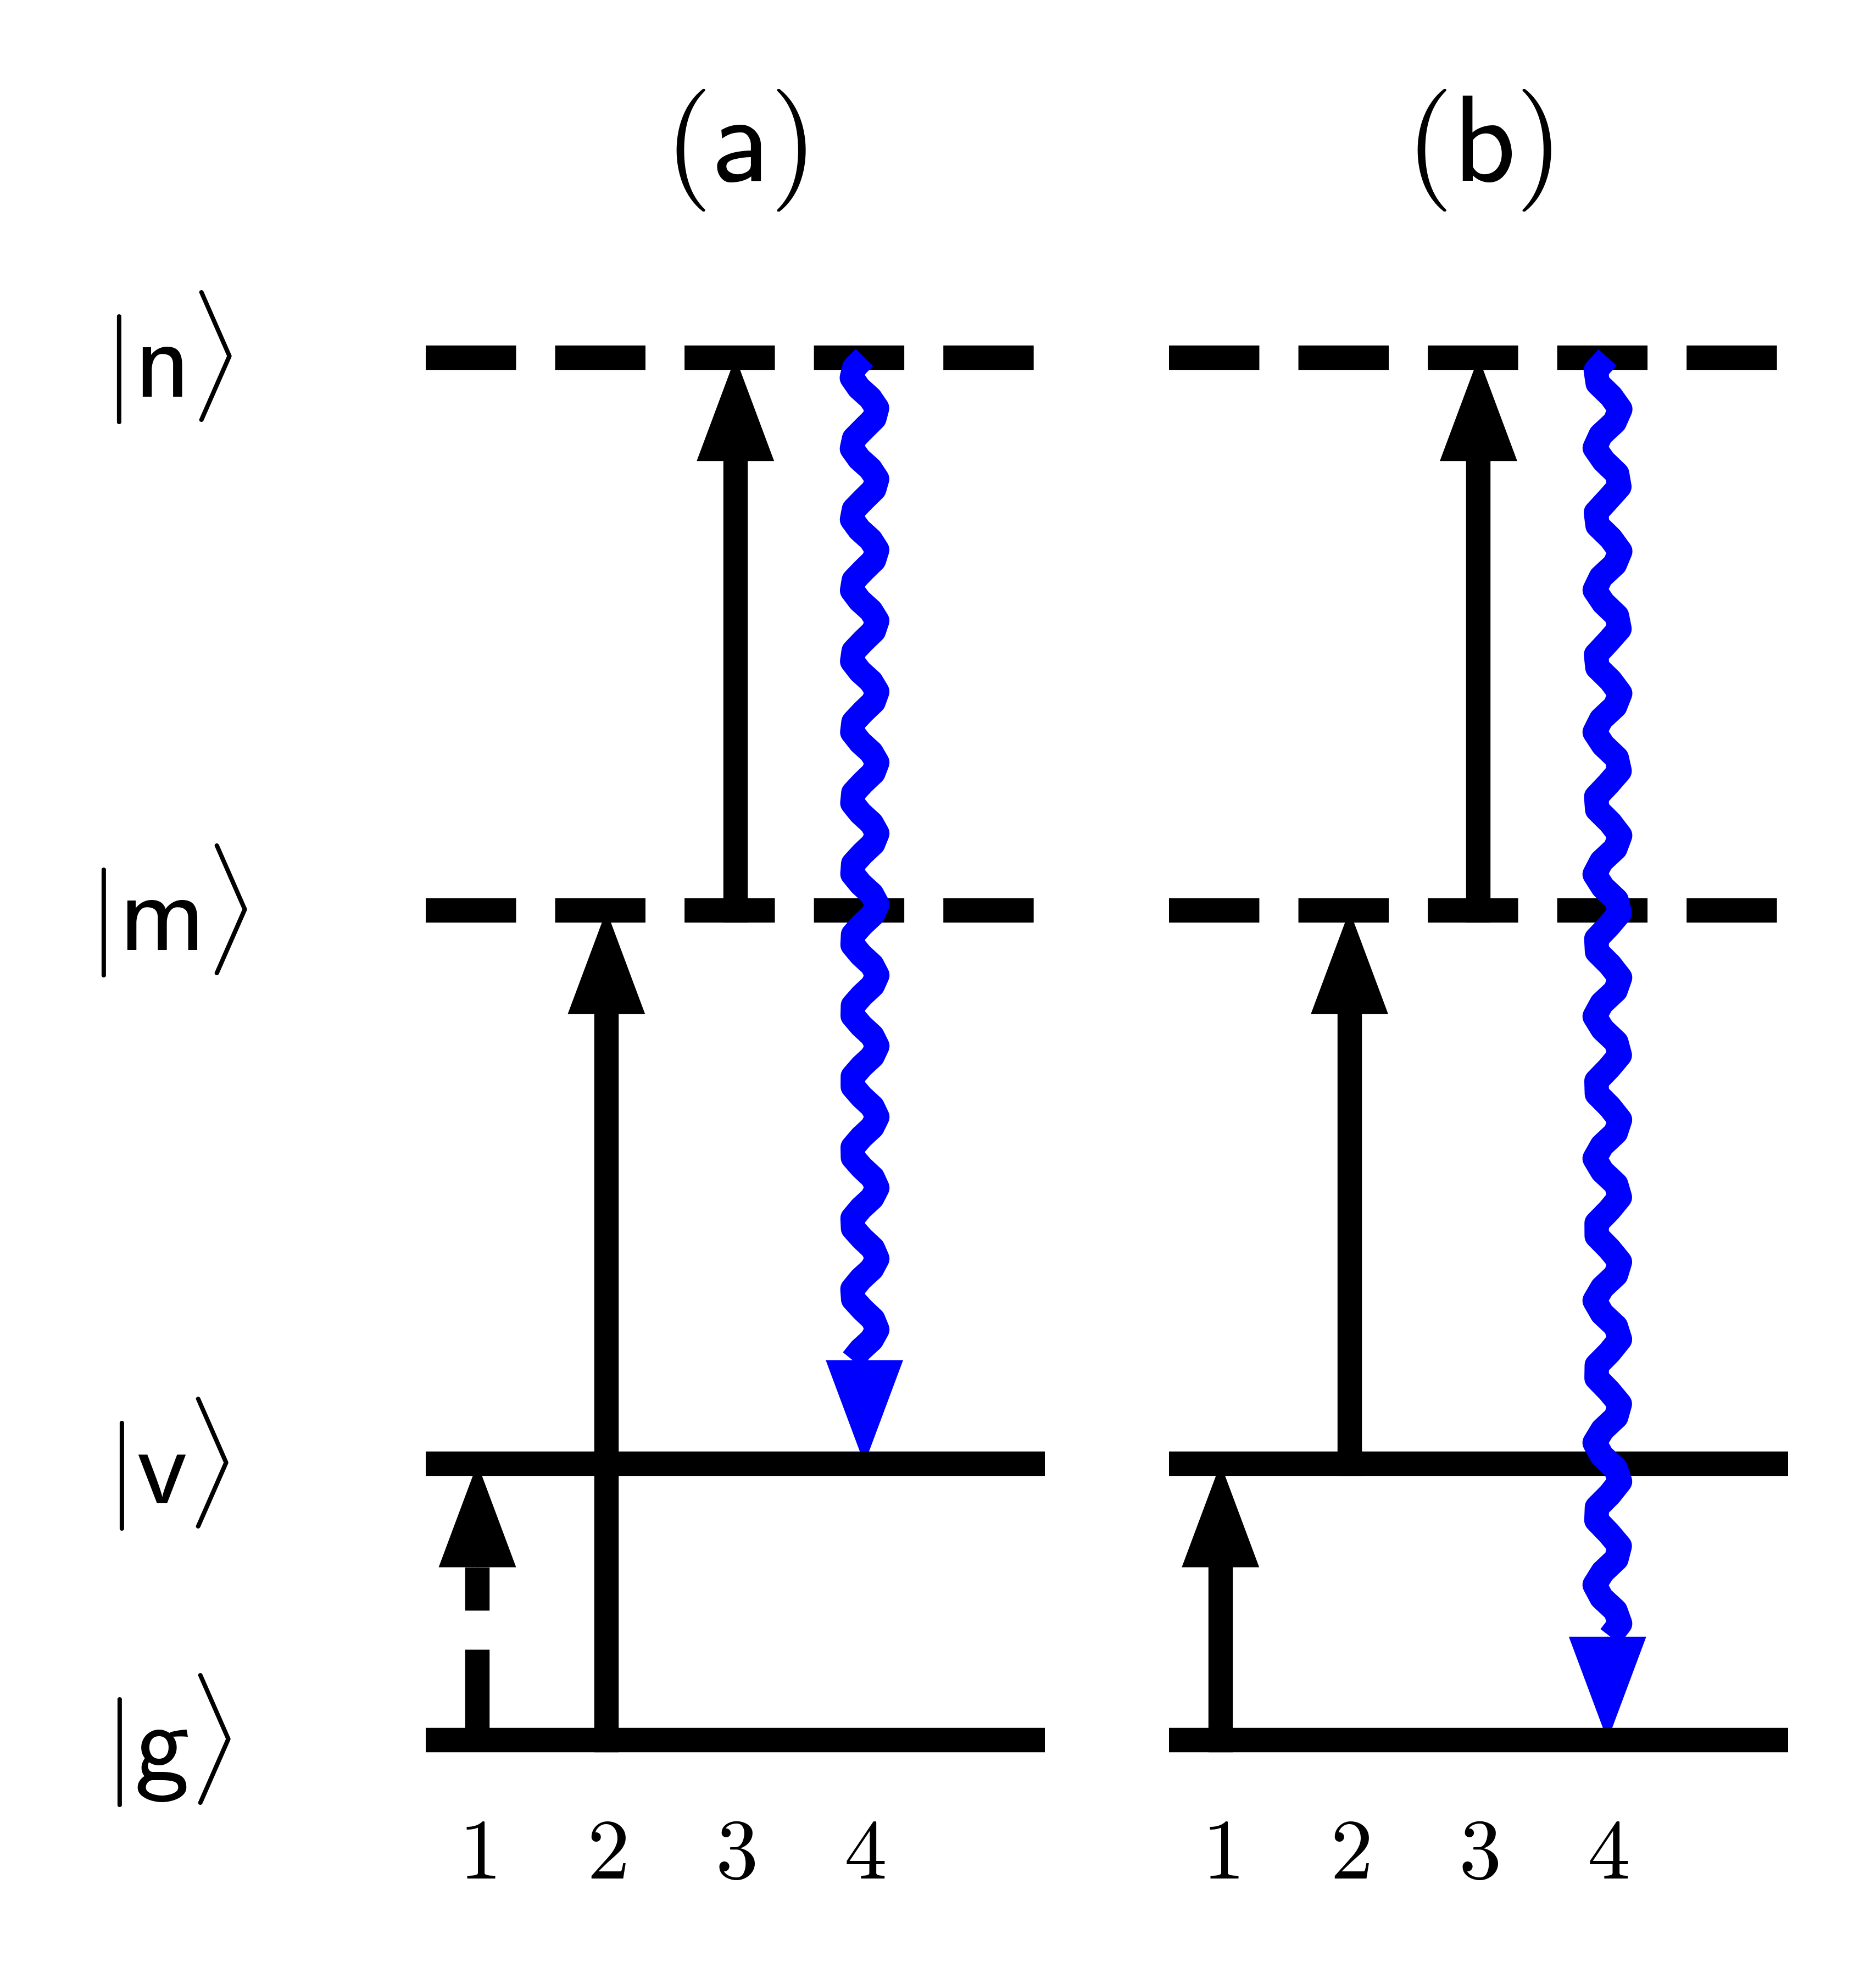
\includegraphics[width=3.375in]{main/wmel1.png}
	\caption{Wave Mixing Energy Level (WMEL) diagrams of the relevant SR-SIVE pathways in the (a) $\vec{k}_4 = -\vec{k}_1 + \vec{k}_2 + \vec{k}_3$ and (b) $\vec{k}_4 = \vec{k}_1 + \vec{k}_2 + \vec{k}_3$ phasematching geometries. \cite{RN286, RN352}
	$\ket{g}$ is the ground state, $\ket{v}$ is an infrared active vibration and $\ket{m}, \ket{n}$ are virtual states.
	Solid and dashed horizontal lines indicate real and virtual states, whereas solid and dotted arrows indicate ket and bra side transitions, respectively. 
	These diagrams can be permuted to generate additional resonant WMEL diagrams.}
	\label{fig:sivewmel}
\end{figure}

It is useful to expose relationships between transition dipoles, Raman polarizabilities and hyper-Raman polarizabilities in the driven limit. \cite{Simpson2004, RN120}
In the driven limit, under the electric dipole approximation, the I$^{th}$ component of the third order nonlinear output polarization, ${P}^{(3)}_I$, of any four wave mixing process, induced by electric fields E, at output frequency $\omega_4$ is written as \cite{RN307}
\begin{equation} \label{polarization}
{P}^{(3)}_I (\omega_4)  = \chi^{(3)}_{IJKL} E_J E_K E_L 
\end{equation}
where $\chi^{(3)}_{IJKL}$ is the IJKL element of the third order electrical susceptibility, a rank four tensor, generally written as
\begin{equation}
	\chi^{(3)}_{IJKL} = NF(\omega_4) \langle \gamma_{ijkl} \rangle
\end{equation}
where N is a number density, F is the Lorentz local field factor, and $\gamma_{ijkl}$ is the third order polarizability (i.e., second hyperpolarizability). 
The brackets indicate an orientational average. 
Uppercase letters refer to laboratory frame coordinates and lower case letters refer to molecular frame coordinates.

Note that we choose the convention where an arbitrary electric field, assuming a plane wave, is written in Fourier components as 
\begin{equation}
	\vec{E}(\omega) = \frac{1}{2} \vec{E}_0 \exp(i(\vec{k}\cdot\vec{x} - \omega t)) + c.c.
\end{equation}
where $E_0$ is the pulse amplitude and $\vec{k}$ is a wavevector.


Expressions for $\gamma_{ijkl}$ can be found by solving Liouville-von Neumann equation for an output density matrix element $\rho_{ij}$.
Generally, under the electric dipole approximation, the density matrix, $\bar{\rho}(t)$, is propagated through the Liouville-von Neumann equation as \cite{RN455}
\begin{equation}\label{matrix}
	\dot{\bar{\rho}}(t) = \frac{1}{i \hbar}[H_0 - \vec{\mu}\cdot \sum_j E_j(\vec{x},t), \bar{\rho}(t)] + \bar{\Gamma} \bar{\rho}(t)
\end{equation} %check if bar or double bar
where $H_0$ is the system (time independent) Hamiltonian, $\vec{\mu}$ is the electric transition dipole moment, $\vec{E}(\vec{x},t)$ is a time dependent electric field, and $\bar{\Gamma}$ is the pure dephasing rate vector. 
In the rotating frame, $\tilde{\rho}_{ij} = \rho_{ij} e^{-i \omega_{ij}t}$.
By solving \autoref{matrix} under steady state ($\dot{\bar{\rho}}(t) = 0$) in the rotating frame, expressions for $\gamma_{ijkl}$ can be readily obtained by multiplying the output dipole moment, $\mu_i$ by the final density matrix element $\rho_{ij}$. 

\subsection{Vibrational SR-SIVE Selection Rules}
To make the connection between SR-SIVE and hyper-Raman scattering, we investigate the gross selection rules of SR-SIVE-IR.
By propagating density matrix elements in the steady state limit, the SIVE hyperpolarizability is \cite{RN119}
\begin{equation}\label{sivegamma}
		\gamma_{ijkl} =	- \sum_{m, n} \frac{1}{\varepsilon_0} \frac{1}{4D} \frac{1}{\hbar^3} \frac{\mu^{i}_{v n} \mu^{j}_{nm} \mu^{k}_{mg} \mu^{l}_{gv} }{\Delta_{nv} \Delta_{mv}\Delta_{gv}}  \rho_{gg}
\end{equation}
where: $\mu^{j}_{ab}$ is the $j^{th}$ element of $\mel{a}{\vec{\mu}}{b}$, $\Delta_{kl} = \omega_{kl} - \omega_{j} - i\Gamma_{kl}$, $\omega_j$ is the frequency of the j$^{th}$ input field, $\Gamma_{kl}$ is the dephasing of $\rho_{kl}$ and $\rho_{gg}$ is the ground state density.
For simplicity, we consider the results for the process diagrammed in \autoref{fig:sivewmel}a, but by multiplying by (-1) and taking a complex conjugate, which arise from the bra-side transition in \autoref{fig:sivewmel}a, results for the \autoref{fig:sivewmel}b  process are obtained.
Note that $\omega_j \rightarrow -\omega_j$ for a bra side transition.
D, the Maker-Terhune degeneracy factor, accounts for permutation symmetry in $\gamma_{ijkl}$ and is defined as $\frac{n!}{(n-m)!}$, where $n$ is the total number of input fields (3 for any four wave mixing experiment) and $m$ is the number of distinguishable input fields.\cite{RN134} 
For a SIVE experiment using two or three distinct input fields, as considered here, D = 6.
Note that $\ket{m}, \ket{n}$ are virtual states (\autoref{fig:sivewmel}).
By contracting over the virtual states to form the hyper-Raman hyperpolarizability $\beta$ (i.e., Placzek approximation), this expression can be simplified immensely.\cite{Long1970} 
Note, however, that if $\omega_2$, $\omega_3$, as depicted in \autoref{fig:sivewmel}, are nearly resonant with any state, the Placzek approximation fails. \cite{Placzek1934, Long1970}
Assuming the validity of the Placzek approximation, \autoref{sivegamma} is written as 
\begin{equation}\label{sivebeta}
	\gamma_{ijkl} =	-\frac{1}{\varepsilon_0} \frac{1}{24 \hbar}\frac{\beta^{(ijk)}_{gv} \mu^{(l)}_{gv}}{\Delta_{gv}} \rho_{gg}
\end{equation}
As such, any mode that is SIVE active must be both hyper-Raman and IR active.
However, since any IR active vibrational mode is hyper-Raman active,\cite{Cyvin1965, Andrews1978} any IR active mode is SIVE active.
This makes SIVE an optically upconverted infrared spectroscopy of isotropic samples, as its selection rules are identically those of IR spectroscopy, but its output is generally in the visible.
Unlike SFG spectroscopy, which is dependent upon both the infrared and Raman activity of a mode (through symmetry constraints, this demands that the microscopic SFG output from centrosymmetric species vanishes),\cite{Shen90, Cotton} SIVE is a nonlinear, optically upconverted spectroscopy for any infrared active mode.

To understand SR-SIVE selection rules more finely, the dipole and first hyperpolarizability operators are Taylor expanded in terms of an n$^{\text{th}}$ normal mode coordinate $Q_n$ about equilibrium: \cite{Long1970}
\begin{subequations}
	\begin{equation}
		\mu = \mu_0 + \frac{\partial \mu}{\partial Q_n} Q_n + \order{\sum_{m,n}{Q_m Q_n}}
	\end{equation}
	\begin{equation}
		\beta = \beta_{0} + \frac{\partial \beta}{\partial Q_n} Q_n + \order{\sum_{m,n}{Q_m Q_n}}
	\end{equation}
\end{subequations}
Substituting into \autoref{sivebeta} gives the SIVE-IR-I hyperpolarizability to $\order{Q_n}$ as \begin{equation}\label{SIVEselection}
		\gamma_{ijkl} =	-\frac{1}{\varepsilon_0} \frac{1}{24 \hbar}  \frac{1}{{\Delta_{gv}}} \ \frac{\partial \beta^{(ijk)}}{\partial Q_n} {\frac{\partial \mu^{(l)}}{\partial Q_n}}  (\mel{g}{Q_n}{v})^2\ \rho_{gg}
\end{equation}
Since this expression is non-zero in the harmonic oscillator limit, SR-SIVE output is allowed for harmonic transitions. 
Similar to SFG, SR-SIVE does not demand anharmonic ground state potential energy surfaces for spectral output. \cite{Shen94, Cho2000}
This selection rule is generally valid for any SR-SIVE process in the $-\vec{k}_1 + \vec{k}_2  + \vec{k}_3$ and $\vec{k}_1 + \vec{k}_2  + \vec{k}_3$ phasematching geometries when the Placzek approximation is valid.

A useful attribute of this selection rule is the added ability of polarization control arising from the hyperpolarizability tensor. 
Similar to polarization control in second harmonic and sum frequency generation experiments which probe different elements of the infrared transition dipole and Raman polarizability tensor,\cite{Heinz1982} probing different elements of the hyperpolarizability tensor in SR-SIVE can greatly assist in understanding ultrafast dynamics in isotropic systems. \cite{Shen90, Bonn2024}
Polarization control in IR-pump-SIVE-probe, analogous to ultrafast transient absorption spectroscopy, would be an interesting venue to assess the sensitivity of SR-SIVE to different hyper-Raman tensor elements.

To motivate the application of SIVE spectroscopy, we perform an approximate calculation to compare the output of parametric SIVE-IR (\autoref{fig:sivewmel}b) to that of vibrational SFG (vSFG) spectroscopy.
Absorption effects are neglected for simplicity.
\begin{widetext}
To allow comparison between the two methods, the output polarizations of each process is written as
	\begin{subequations}
		\begin{equation}
			\abs{P^{(2)}_{\text{SFG}}} = N_{surf} F(\omega_1+\omega_2) \abs{\langle \alpha_{ij}\mu_{k} \rangle E_J(\omega_2)E_K(\omega_1)} 
		\end{equation}
		\begin{equation}
			\abs{P^{(3)}_{\text{SIVE}}} = N_{bulk}  F(\omega_1+\omega_2 +\omega_3) \abs{\langle \beta_{ijk} \mu_{l} \rangle E_J{(\omega_3)}E_K(\omega_2)E_L(\omega_1)} \ell_{eff}
		\end{equation}
	\end{subequations}
where $\alpha_{ij}$ is the Raman polarizability, N$_{bulk}$ is the bulk number density, and N$_{surf}$ is the surface number density (10$^{19}$ m$^{-2}$).\cite{RN133, RN503}	
\end{widetext}
For liquids with molar masses less than $\sim$100 g mol$^{-1}$ and densities roughly equal to that of H$_2$O$_{(l)}$ at room temperature, N$_{bulk} \sim$ 10$^{28}$ m$^{-3}$.
We take the bulk optical interaction length ($\ell_{eff}$) to be 10 $\mu$m.\cite{RN133} %see chapter 25 of Shen's NLO book... idk something here seems wrong
A normal dispersion curve is assumed so that $F(\omega_1+\omega_2) \approx F(\omega_1+\omega_2 +\omega_3)$.
To simplify analysis, orientational averaging is ignored (e.g., $\langle \beta_{ijk} \mu_{l} \rangle \approx \beta \mu$) and the input and output fields are taken to be co-polarized, so that
\begin{equation}
		P_{ratio} \equiv \frac{\abs{P^{(3)}_{\text{SIVE}}}}{\abs{P^{(2)}_{\text{SFG}}}} \approx \frac{N_{bulk}}{N_{surf}} \frac{\beta}{\alpha} E(\omega_3) \ell_{eff} \sim 10^4 \frac{\beta}{\alpha} E(\omega_3)\\
\end{equation}
Ziegler has noted that for a field of intensity 10 GW/cm$^{2}$, $\frac{\beta E}{\alpha} \sim 10^{-3} $ for vibrational modes when $E(\omega_3)$ is largely detuned from electronic resonances. \cite{RN515}
Such an intensity is easily obtained using modern ultrafast sources.
As such,
\begin{equation}
\begin{split}
		P_{ratio} &\sim 10^4 \frac{\beta E(\omega_3)}{\alpha} \sim 10
\end{split}
\end{equation}
Since the intensity ratio scales as $\abs{P_{ratio}}^2$, we see that the SIVE output is roughly 100 times stronger than vibrational SFG.
It is important to note that this derivation ignored absorption and orientational averaging effects, which can significantly reduce output from either process. 

\subsection{Rovibrational SR-SIVE Selection Rules} %this can probably be deleted but wanted to add just in case...
Recent developments in nonlinear spectroscopy have demonstrated the feasibility of multidimensional infrared spectroscopy of gaseous and quasi-free species. \cite{Ziegler2018, Gronborg2022, RN325, Chen2024}
DOVE and 2D-IR have been used to isolate coupling between fundamentals, overtones and combination bands of gaseous species in several molecular systems. 
Since resonance hyper-Raman scattering spectroscopy was developed as a gas phase spectroscopy,\cite{RN515} we briefly investigate the properties of rovibrational SR-SIVE.

The rovibrational selection rules are generated through calculating \autoref{sivebeta} in a $\ket{vJM} \equiv \ket{v} \otimes {\ket{JM}}$ basis, where $\{\ket{v}\}$ is a basis of vibrational states and $\{\ket{JM}\}$ is a basis of rotational states ($J$ is the rotational quantum number and $M$ is its z projection, respectively).
By writing $\vec{\mu} = T_{q_1}^{(1)}$ and $\beta_{ijk} = T_{q_1}^{(1)} + T_{q_2}^{(2)} + T_{q_3}^{(3)}$, where $T^{(k)}_{q}$ is a rank $k$ spherical tensor, it is simple to evaluate the integrals in \autoref{sivebeta} through the Wigner-Eckart theorem. \cite{Kowzan2022}
It is important to note that $\beta_{ijk}$ does not have complete tensor index symmetry.
Specifically, it has shown that the rank one spherical tensor ($T_{q_1}^{(1)}$, with $q_1 \in \{-1, 0 ,1\}$) fully contributes to $\beta_{ijk}$ but only select $T_{q_2}^{(2)} + T_{q_3}^{(3)}$ terms contribute. \cite{Andrews1978, Andrews1990}
%there is some fancy way to note that theres no index constraint but i dont remember the language...
As such, its decomposition into irreducible tensor form is allowed only if the values of $q', q''$ are constrained.
By substituting the spherical tensor definitions of $\vec{\mu}$ and $\beta_{ijk}$ into \autoref{sivebeta}, it is clear that only $\Delta J = \pm 1$ transitions are allowed, i.e., SIVE-IR features arise only from P or R branches (assuming the ground state is $\ket{g00}$).
This is expected since $\vec{\mu}$ transitions demand $\Delta J = \pm 1$.
As a result, consistent with vibrational SR-SIVE, rovibrational SR-SIVE follows the same rules as common infrared rovibrational spectroscopy.

\subsection{Quantitative SR-SIVE}
With the selection rules of SR-SIVE understood for vibrational and rovibrational spectroscopy, it becomes possible to extract quantitative information from SIVE spectra to compare to incoherent methods and other CMDS methods.

Lineshape analysis is essential for extracting quantitative information from CMDS spectra.
Scanning across resonances create dispersive lineshapes, i.e, self-heterodyning, which inform on $\Re{\chi^{(3)}}$ and $\Im{\chi^{(3)}}$.\cite{Levenson1974_1, Levenson1974_2}
Resonant SIVE lineshapes are complicated by amplitude level interference between the sample and its substrate and/or sample cell windows. \cite{RN362}
These effects have been treated in excellent detail for three laser infrared-infrared-visible SIVE using the pathway in \autoref{fig:sivewmel}a, and provide methods to export quantitative information from SIVE spectra. \cite{RN418}

Most quantitative methods in an n$^{th}$ order CMDS experiment are used to extract $\chi^{(n)}$ values for comparing the relative strength of nonlinear processes in different media. \cite{Zhu87, RN351, RN345}
The recorded $\chi^{(n)}$ values provide insight into how microscopic quantities ($\vec{\mu}, \alpha_{ij}, \beta_{ijk}$) impact nonlinear output.
To our knowledge, only 2D-IR spectroscopy has taken advantage of orientationally averaged $\chi^{(3)}$ values to extract transition moments. \cite{Moilanen2009, RN245}
Previous treatments did not consider using quantitative analysis in SIVE to measure $\beta_{ijk}$ values from SIVE spectra.
It is thus useful to investigate how a simple treatment of orientational averaging can extract $\beta_{ijk}$ from a $\chi^{(3)}_{IJKL}$ expression.

The SIVE $\chi^{(3)}_{IJKL}$ expresson is
\begin{equation}\label{chi3}
\begin{split}
		\chi^{(3)}_{IJKL} &\sim \langle \gamma_{ijkl} \rangle \sim \langle \beta_{ijk} \mu_l \rangle\\
\end{split}
\end{equation}
The steps behind orientational averaging of $\gamma_{ijkl}$ are detailed elsewhere.\cite{Andrews1977, McDonnell2024}
Orientational averaging for specific input polarizations shows that specific polarization schemes isolate linear combinations of different $\beta_{ijk}$ terms. 
Infrared spectra can provide values for different $\vec{\mu}$ components.
Since $\vec{\mu}$ is a rank-one tensor, its three Cartesian components share the simple relationship $\langle {\mu^2_x} \rangle = \langle {\mu^2_y} \rangle = \langle {\mu^2_z} \rangle = \frac{1}{3}\langle {\mu^2} \rangle$. \cite{RN459}
Neglecting rotational dependence, $\langle {\mu^2} \rangle = \abs{\mu}^2 = \mu^2$.
Substituting into \autoref{chi3} shows that
\begin{subequations}
	\begin{equation}
		\begin{split}
			\chi^{(3)}_{IJKL} &\sim \langle \beta_{ijk} \mu_l \rangle\\
			&\sim \langle \beta_{ijk} \rangle \frac{\mu}{\sqrt{3}} 
		\end{split}
	\end{equation}
This is done because any element of $\vec{\mu}$ is easily related to its magnitude through the directional cosine relationship shown above. 
Continuing, we see
	\begin{equation}
		\langle \beta_{ijk} \rangle \sim \frac{\sqrt{3}}{\mu} \chi^{(3)}_{IJKL}
	\end{equation}
\end{subequations}
Since $\mu^2$ can be extracted by fitting infrared spectra,\cite{RN412} it is clear that different polarization schemes in SIVE spectroscopy give a measurement of $\beta_{ijk}$ values.
SIVE can therefore provide useful insight into the sensitivity of hyper-Raman spectroscopy to different infrared active vibrations.
 

\subsection{Coherent Interference in SR-SIVE}
It is well known that nonlinear wave mixing processes which share the same time ordering and output frequency will interfere. \cite{RN135, Bonn2024}
Understanding interfering pathways is useful because they can, in some cases, eliminate output. \cite{RN342, RN135}
The WMEL diagrams presented in \autoref{fig:sivewmel} outline resonant SIVE processes when the infrared pulse $(\omega_1)$ is resonant with a vibrational mode. 
However, if $\omega_2$ becomes vibrationally resonant and $\omega_1$ is non-resonant, then other SIVE pathways appear.\cite{McDonnell2024} 
While the methods in \autoref{fig:sivewmel2} possess identical selection rules to \autoref{fig:sivewmel}, the WMEL diagrams presented in \autoref{fig:sivewmel2} may significantly interfere with DOVE-IR and DOVE-Raman spectra.
The time ordering in DOVE-IR and DOVE-Raman spectra is used to interpret anharmonicities, as DOVE-IR and DOVE-Raman destructively interfere when outputs are at the same frequency. \cite{RN135, RN324}
It is therefore important to understand how the corresponding SIVE pathways interfere.
To this end, we investigate how the SIVE-IR-II and SIVE-Raman pathways (\autoref{fig:sivewmel2}a, b, respectively) interfere under the rotating wave approximation. 

\begin{figure}[!htbp]
	\centering
	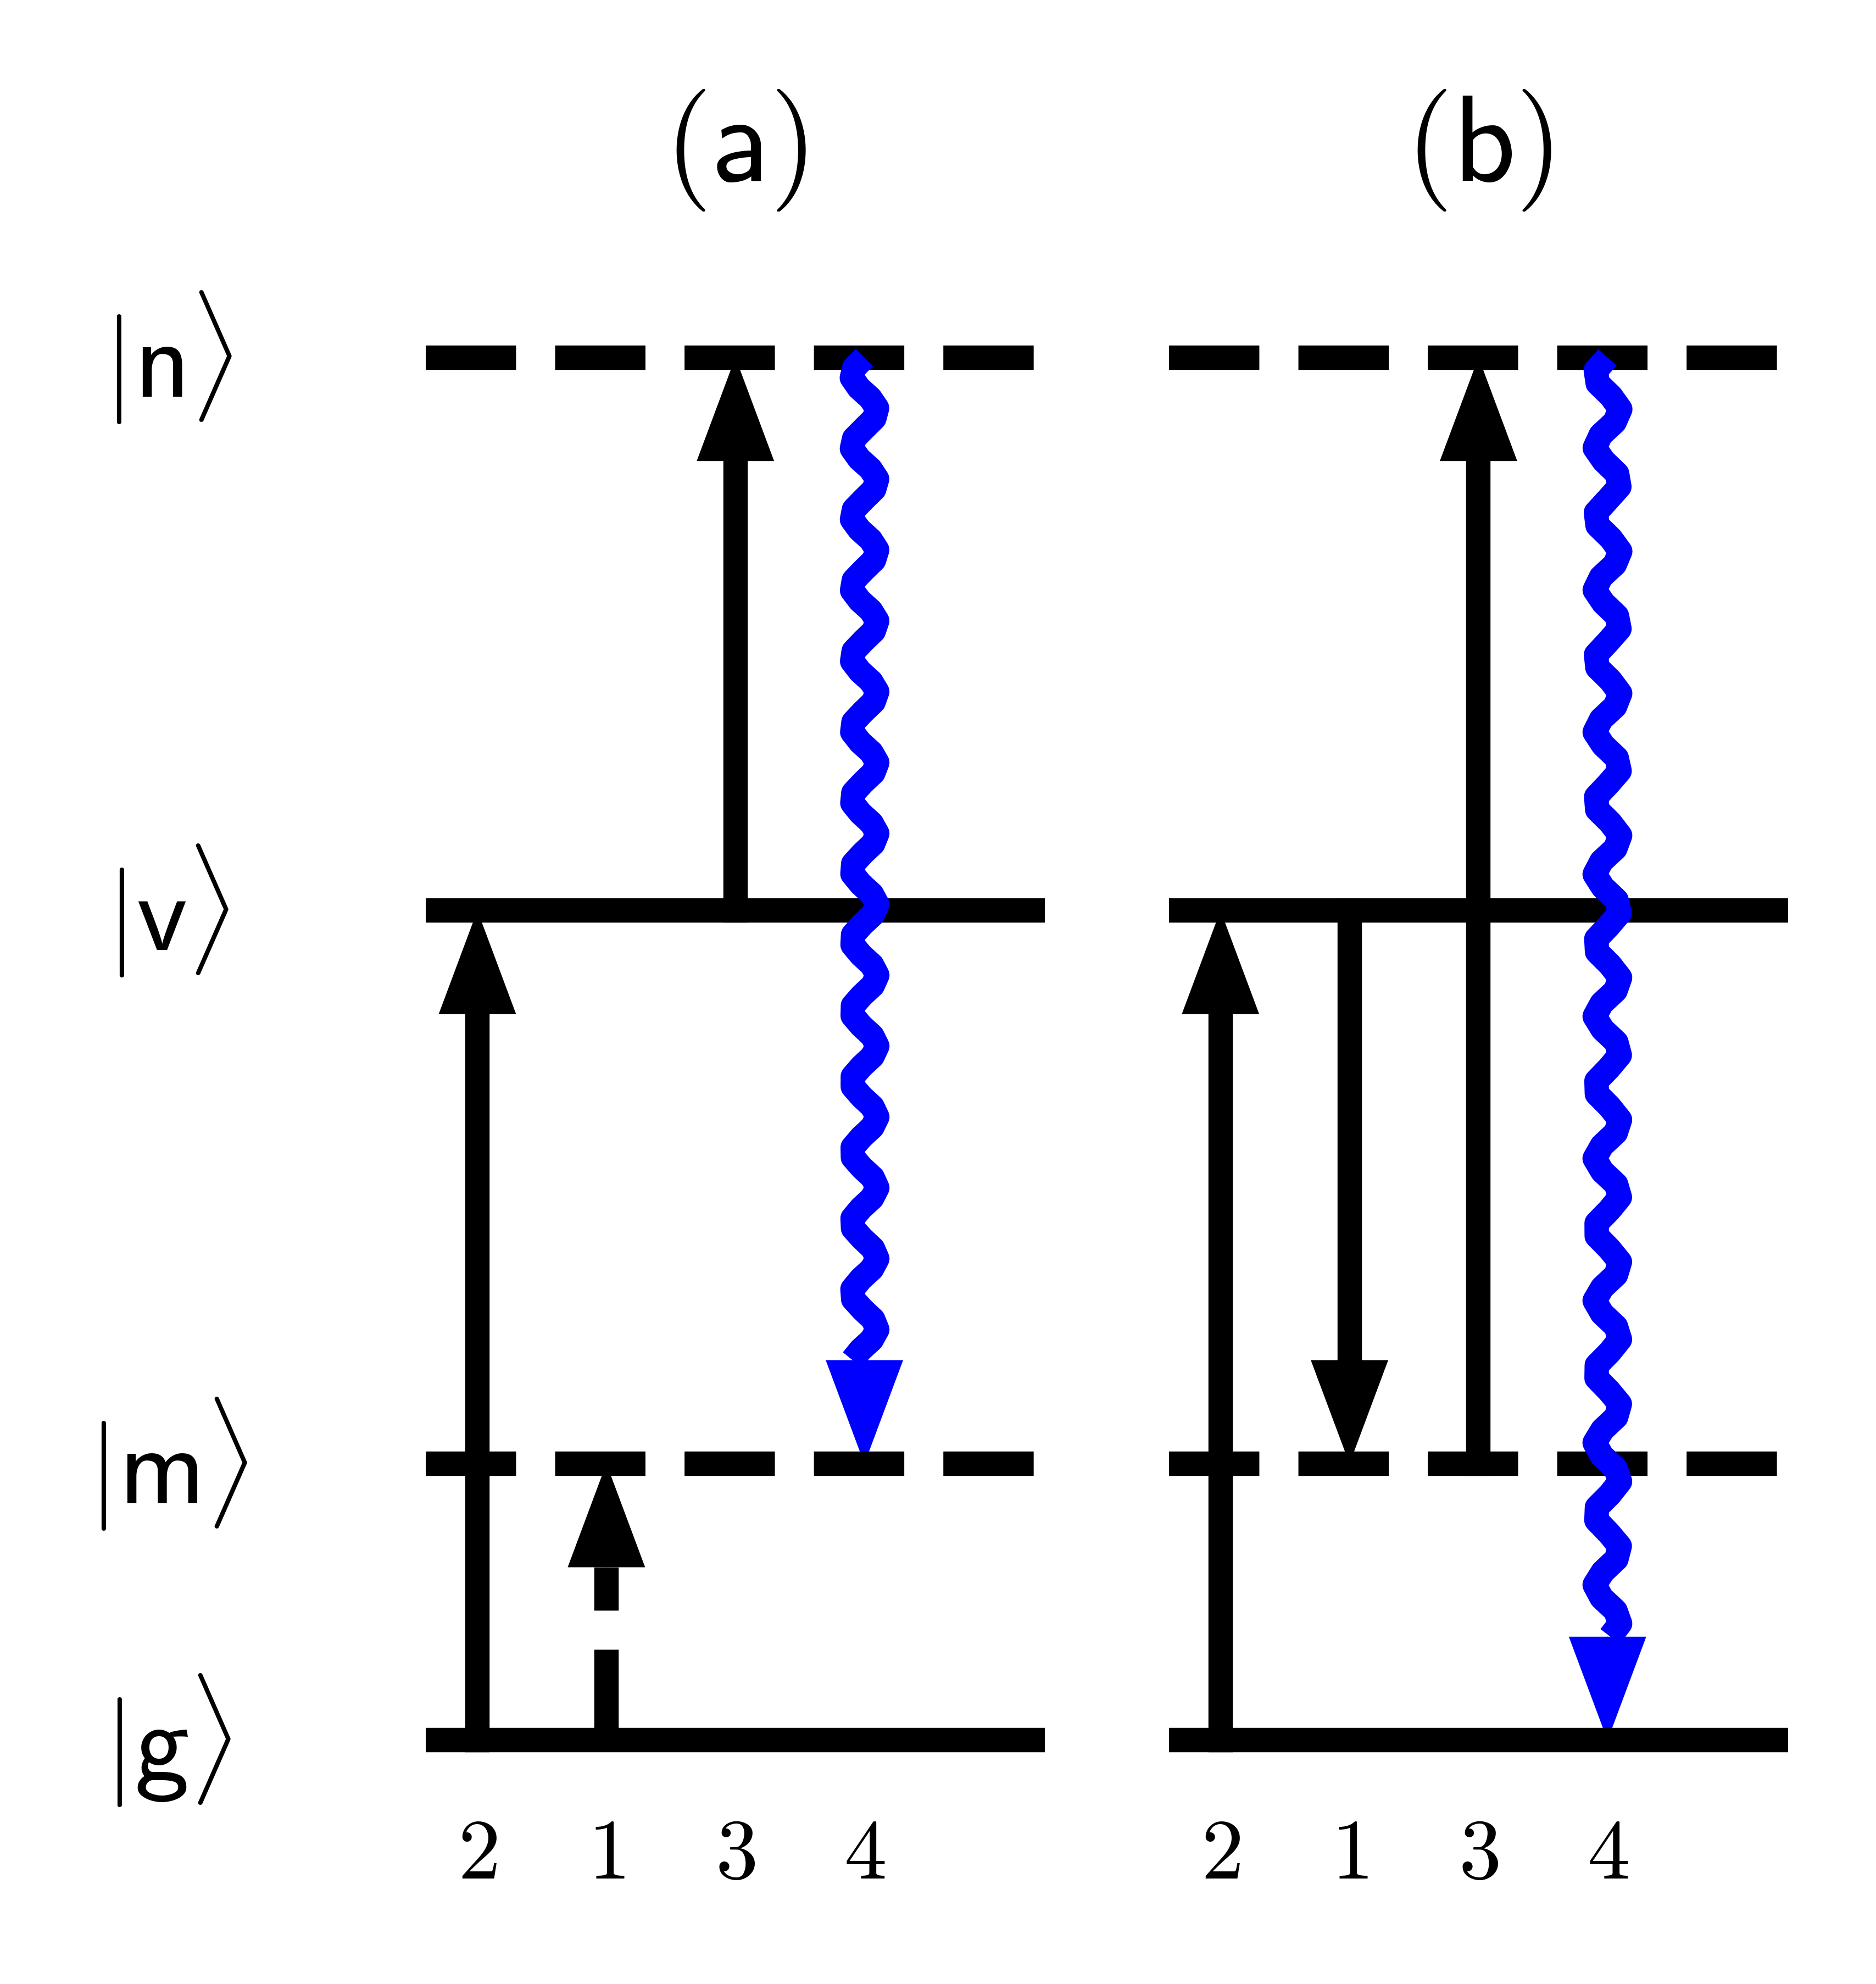
\includegraphics[width=3.375in]{main/wmel2.png}
	\caption{Wave Mixing Energy Level (WMEL) diagrams of interfering SR-SIVE pathways in the  $\vec{k}_4 = -\vec{k}_1 + \vec{k}_2 + \vec{k}_3$ phasematching geometry. 
	(a) is similar to the process diagrammed in \autoref{fig:sivewmel}, whereas (b) is similar to a singly resonant coherent anti-Stokes Raman-type process.}
	\label{fig:sivewmel2}
\end{figure}
\begin{widetext}
We employ the response function formalism of Mukamel for this analysis. \cite{RN287}
The third order response functions, $R^{(3)}$, for SR-SIVE-IR-II ($R^{(3)}_{S_{II}}$) and SR-SIVE-Raman ($R^{(3)}_{R}$) (\autoref{fig:sivewmel2}a, b) are 
\begin{subequations}
	\begin{equation} \label{mixing:a}
		R^{(3)}_{S_{II}} (t_2) = -\frac{i}{\hbar} [\beta(t_2), \mu(0)] \exp(-i\Delta_{v''g}t_2) \theta(t_2)
	\end{equation}
	\begin{equation}\label{mixing:b}
		\begin{split}
			R^{(3)}_{R} (t_2) & = \frac{i}{\hbar} [\beta(t_2), \mu(0)] \exp(-i\Delta_{v''g}t_2) \theta(t_2) = - R^{(3)}_{S_{II}} (t_2)\\
		\end{split}
	\end{equation}
\end{subequations}
By assuming that the beams which stimulate hyper-Raman scattering, $\vec{E}_1, \vec{E}_3$, interact simultaneously at some time $\tau$ after $\vec{E}_2$ interacts with the sample, the total output polarization, $\vec{P}^{(3)}(t)$, is written as \cite{Cho2001}
	\begin{equation}\label{polarization_SRSIVE_a}
		\begin{split}
			\vec{P}^{(3)}(t) &= \vec{P}_{S_{II}}(t) + \vec{P}_{R}(t)\\
			&= \int_0^\infty \mathrm{d}t_2 (R^{(3)}_{S_{II}} (t_2) + R^{(3)}_{R} (t_2))\vdots \vec{E}_3(t) \vec{E}_1(t) \vec{E}_2(t-t_2 + \tau)\\
			&= \int_0^\infty \mathrm{d}t_2 (R^{(3)}_{S_{II}} (t_2) - R^{(3)}_{S_{II}} (t_2))\vdots \vec{E}_3(t) \vec{E}_1(t) \vec{E}_2(t-t_2 + \tau) \\
			&= 0
		\end{split}
	\end{equation}
It is clear the total output polarization for SR-SIVE-IR-II and SR-SIVE-Raman vanishes, or, SR-SIVE-IR-II and SR-SIVE-Raman perfectly destructively interfere.
\end{widetext}
The absence of SR-SIVE-IR-II pathways in ultrafast DOVE work is rationalized by this calculation. \cite{RN367, McDonnell2024}
In the case of the time ordered SR-SIVE-IR-I pathway, there are no opportunities for interference as all other pathways are nonresonant with the first interaction. 
A possible mechanism for interfering output in the SR-SIVE-I pathway are cascaded second order processes (SFG, DFG). \cite{RN243, RN300}
In isotropic media, SFG and DFG vanish under the electric dipole approximation,\cite{Zhu87} so cascades are unlikely to inhibit output in centrosymmetric media.
In media where SFG and DFG are allowed, e.g. surfaces or noncentrosymmetric media, second order cascades may become important. 
Generally, for nonlinear spectroscopies which share the same phasematching conditions as SR-SIVE (e.g., DOVE), it is useful to note that SR-SIVE-IR-I is not canceled, whereas SR-SIVE-IR-II and SR-SIVE-Raman permanently cancel.

\begin{figure}[!htbp]
	\centering
	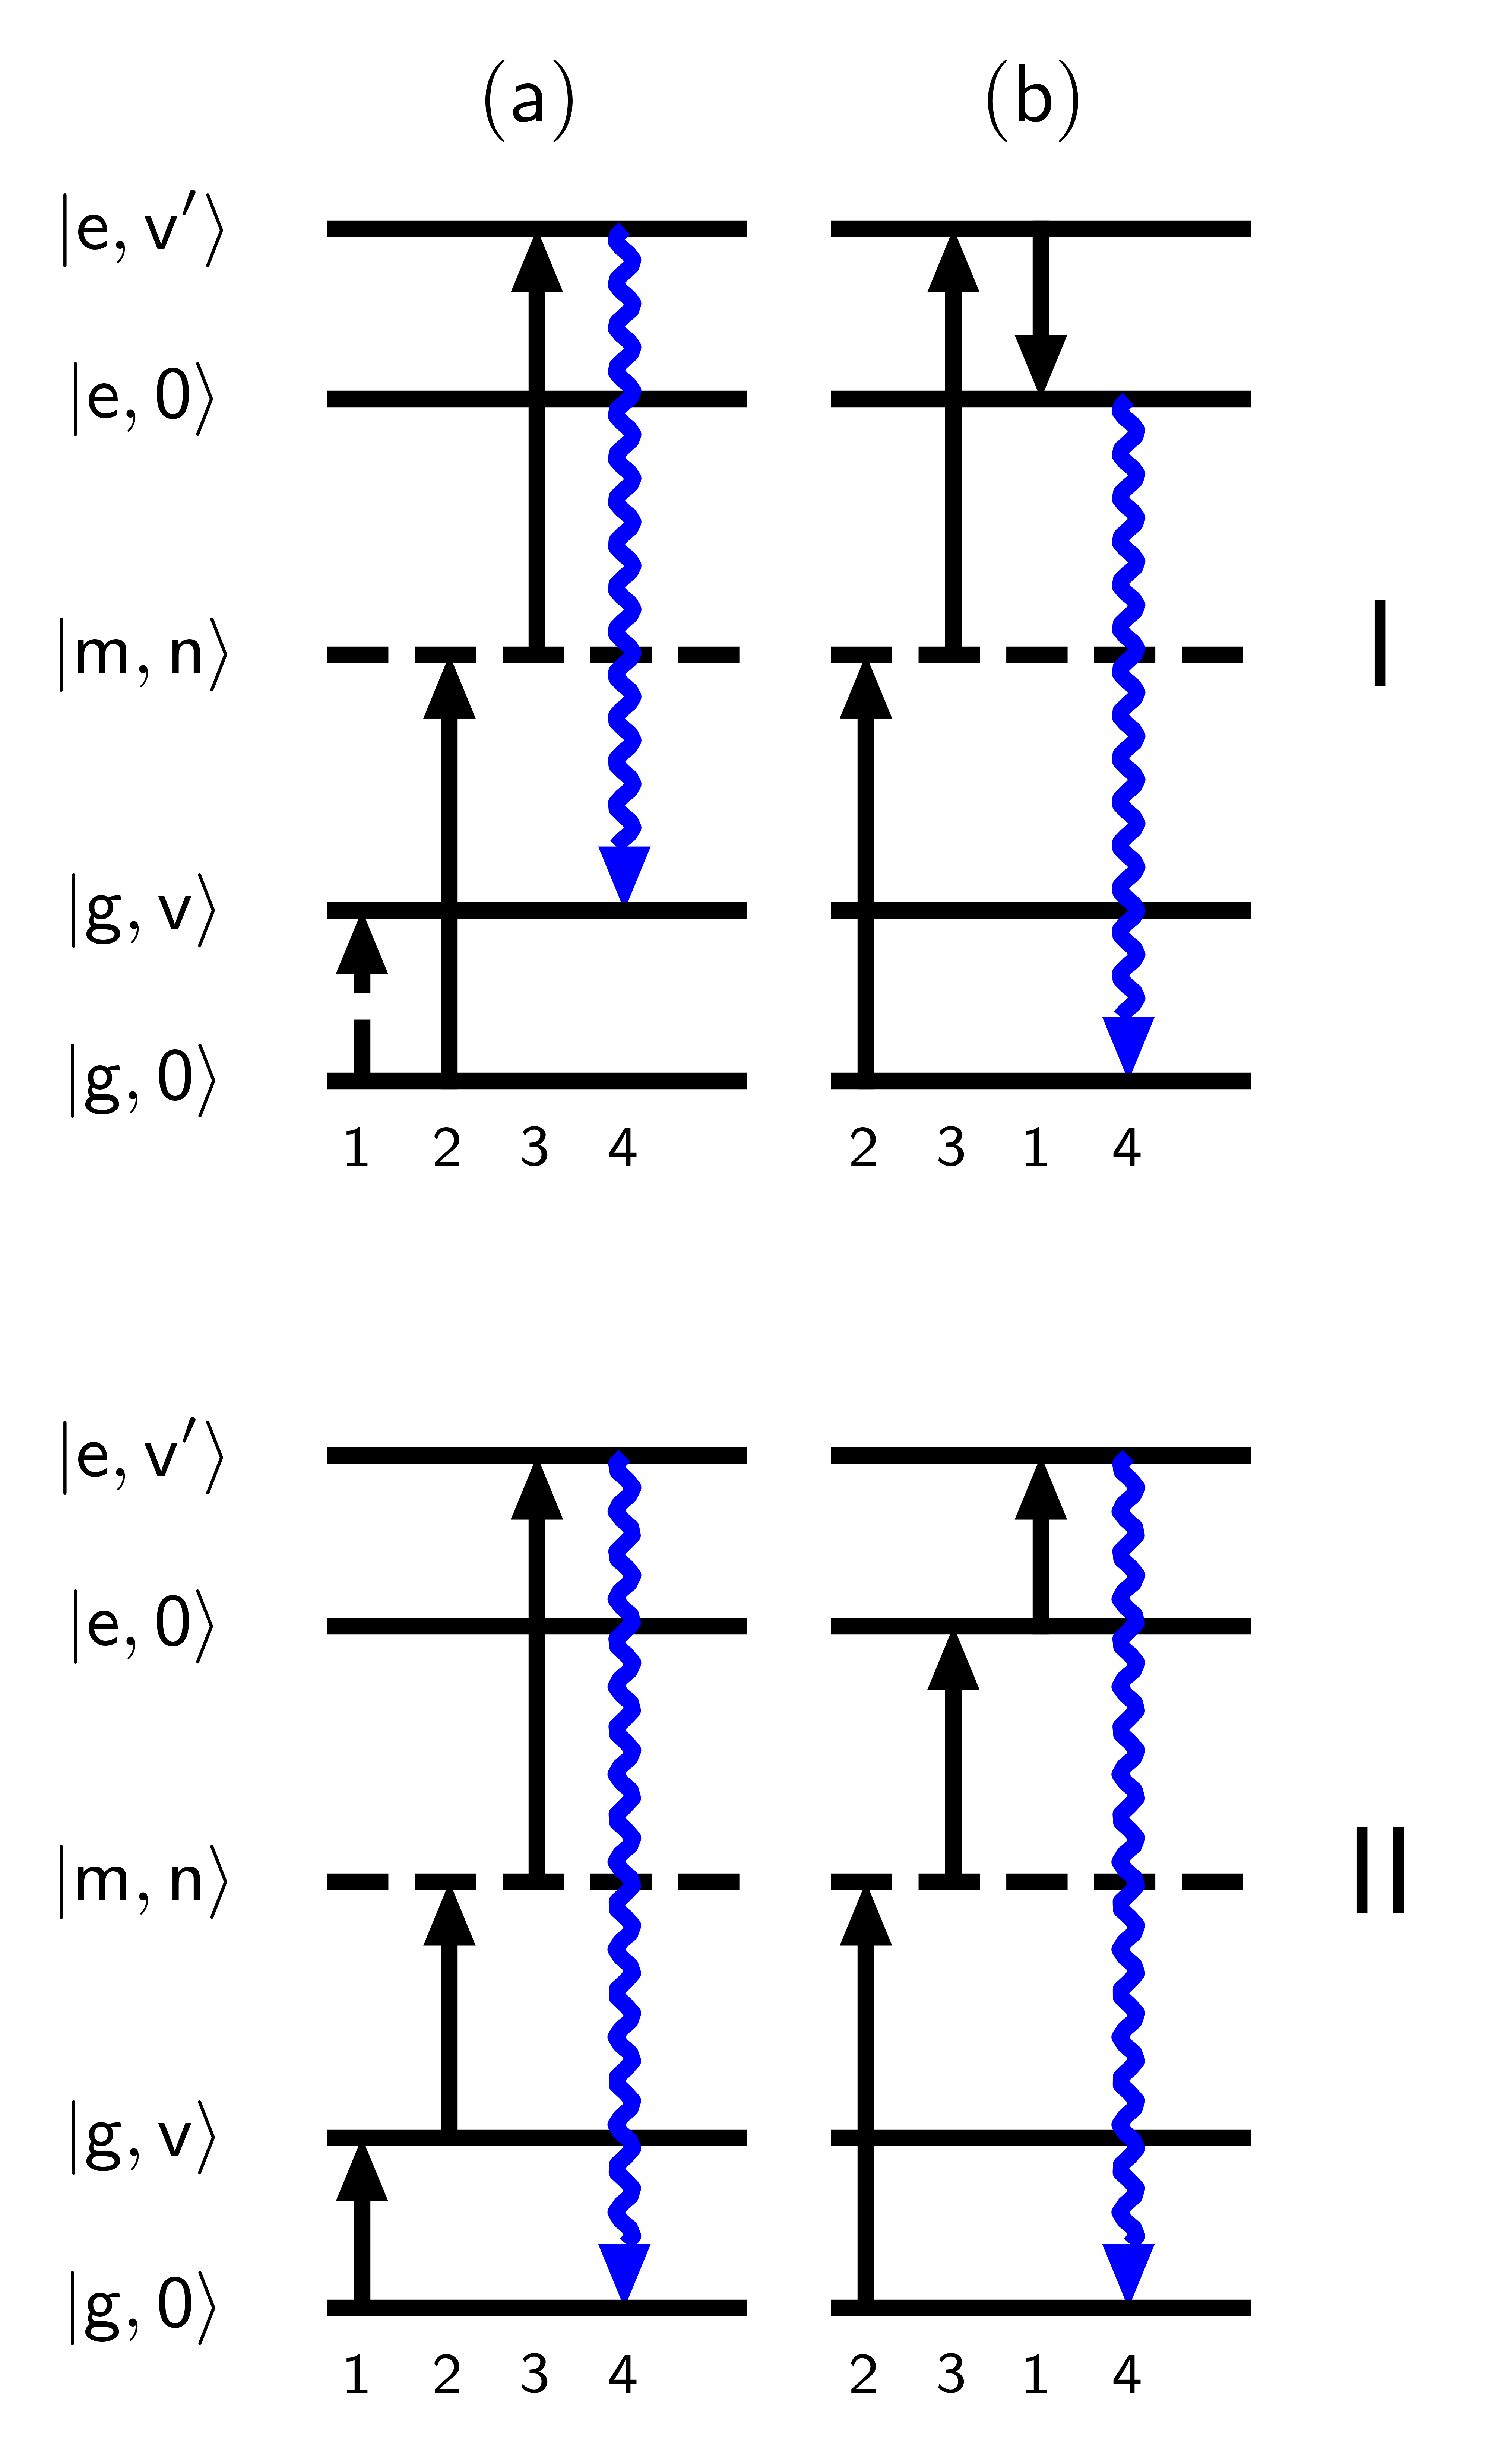
\includegraphics[width=3.375in]{main/wmel3.png}
	\caption{WMEL diagrams of some DR-SIVE pathways in the $-\vec{k}_1 + \vec{k}_2+ \vec{k}_3$  (I-a,I-b) and $\vec{k}_1 + \vec{k}_2+ \vec{k}_3$ (II-a,II-b) phasematching outputs. $\ket{g,0}$ denotes the ground states, $\ket{g,v}$ denotes a vibrational state on the ground electronic manifold; $\ket{m,n}$ denotes a virtual state, and $\ket{e,0}, \ket{e,v'}$ denote vibronic states.}
	\label{fig:doubsive}
\end{figure}

\subsection{DR-SIVE-IR Selection Rules} %%most of this can probably be scrapped because... we don't really learn much new here.
DR-SIVE (where a vibrational and vibronic state are resonantly coupled) can provide a tool for measuring vibronic coupling.
This method is analogous to doubly resonant sum frequency generation. \cite{Shen94}
Multi-resonant nonlinear spectroscopies, such as coherent anti-Stokes Raman spectroscopy (CARS), 2D Electronic Vibrational (2D-EV) spectroscopy and triply resonant sum frequency generation (TRSF) spectroscopy, have been employed to resolve vibronic coupling in molecular samples. \cite{Carlson1990, Gaynor2017, RN276}
DR-SIVE provides methods to investigate vibronic coupling with only two laser pulses, as long as the electronic state is accessible via two photon absorption from the ground state (\textit{vide infra}).
Two beam, parametric and non-parametric DR-SIVE processes are diagrammed in \autoref{fig:doubsive}.
Here, states are written assuming the Born-Oppenheimer approximation, such that $\ket{a,b} = |a) \otimes \ket{b}$ for electronic states $\{|a)\}$ and vibrational states $\{\ket{b}\}$. \cite{BornOppenheimer, Albrecht1960}

The goal of this section is to understand DR-SIVE-IR selection rules.
We begin by inspecting the selection rules of a non-parametric DR-SIVE pathway (\autoref{fig:doubsive}I-a) in the driven limit. 
The driven limit is useful as despite the sum over states approach, it avoids implications of ultrafast dephasing of the vibronic state.\cite{Cho2001} 
For consistency with previous reports, we use $\vec{R}$ to denote electric transition dipole moments (not to be confused with the response function; $\mu$ is used for transitions between states on the ground electronic state.). \cite{Ziegler1974}
Following the approach which gave \autoref{sivegamma}, we find
\begin{equation}\label{drgamma_notaylor}
	\gamma_{ijkl} = -\frac{1}{\varepsilon_0} \frac{1}{24 \hbar^3} \sum_{m,n,v'} \frac{
		R^{i}_{gv,ev'} 
		R^{j}_{ev',mn} 
		R^{k}_{mn,gv} 
		R^{l}_{gv,g0} 
	}{\Delta_{g0,gv}
		\Delta_{ev', mn}
		\Delta_{mn, g0}
	}
\end{equation}
where $R^{i}_{gv,ev'}$ is the i$^{th}$ element of $\mel{g,v}{\vec{R}}{e,v'}$.
For generality, we assume that the vibronic  $\ket{e,v'}$ does not share the same vibration with $\ket{g,v}$. \cite{Ziegler1988}
Using our definition of vibronic states, we write $\vec{M}_{ab} = (a|\vec{M}|b)$ so that, for example,
$R^{i}_{gv,ev'} = \mel{v}{M^i_{ge}}{v'}$.\cite{Albrecht1960}
\begin{widetext}
Using these ideas rewrites \autoref{drgamma_notaylor} as
\begin{equation}\label{drgamma_notaylor_1}
	\gamma_{ijkl} = -\frac{1}{\varepsilon_0} \frac{1}{24 \hbar^3} \sum_{m,n,v'} \frac{
		\mel{v}{M^{i}_{ge}}{v'} 
		\mel{v'}{M^{j}_{em}}{n}
		\mel{n}{M^{k}_{mg} }{v}
		\mel{v}{M^{l}_{gg}}{0}
	}{\Delta_{g0,gv}
		\Delta_{ev', mn}
		\Delta_{mn, g0}	}
\end{equation}
Contracting over $m,n$ in \autoref{drgamma_notaylor_1} by invoking the two photon absorption polarizability $\Lambda$ gives \cite{McClain1977, Simpson2004, Olson2018}
\begin{equation}\label{drgamma_alpha_0}
	\gamma_{ijkl} = -\frac{1}{\varepsilon_0} \frac{1}{24 \hbar^2} \sum_{v'} \frac{
		\mel{v}{M^{i}_{ge}}{v'} 
		\mel{v'}{\Lambda^{jk}_{eg}}{v}
		\mel{v}{M^{l}_{gg}}{0}
	}{\Delta_{g0,gv}
		\Delta_{ev', g0}
	}
\end{equation}
where ${\Lambda^{jk}_{eg}} = (e|\Lambda^{jk}|g)$. 
\end{widetext}
Since $\Lambda^{jk}$ transforms like a rank two tensor, it is clear that the electronic transition must be both one and two photon allowed for non-zero output, similar to resonant second harmonic generation spectroscopy. \cite{Heinz1982, Nguyen1986, Simpson2004}
This is identical to a selection rule in resonance hyper-Raman scattering, as derived by Chung and Ziegler. \cite{Ziegler1988}
As such, the DR-SIVE methods discussed here are coherent, resonance hyper-Raman analogues. 
This makes DR-SIVE a type of resonance IR spectroscopy, as introduced by Boyle et al.\cite{RN491} 
However, in the methods described by \autoref{drgamma_alpha_0}, $|e)$ must be accessible through one and two photon transitions from $|g)$.
Conversely, the resonance-IR method demonstrated by Boyle et al. only requires one photon transitions between $|g)$ and $|e)$.
Systems which provide strict parity induced selection rules (e.g., benzene) will be useful for assessing the validity of these selection rules and comparing the method described here and that of Boyle et al. \cite{RN491}

\subsection{Line Narrowing in SIVE Spectroscopies}
An unavoidable consequence in electronic spectroscopy is broadened lineshapes due to the inhomogeneity of electronic transitions (e.g., vibronic sidebands, molecular collisions). 
Four wave mixing methods can line-narrow transitions and remove some impact of inhomogeneous broadening.\cite{Carlson1990line}
The line-narrowing properties of DR-SIVE are investigated so that the pathways which line-narrow correlated or anti-correlated modes (\textit{vide infra}) can be identified.
SR-SIVE cannot linenarrow transitions as it is singly resonant. \cite{RN352}

In the discussion that follows, we assume that a vibrational mode in the ground state, $\ket{g,v}$, is correlated to the frequency of a vibronic $\ket{e,v}$.\cite{Carlson1990}
If the frequency of $\ket{g,v}$ is written as $\omega_{gv} + \xi$, where $\xi$ is some external strain (e.g. molecular collisions), then the frequency of $\ket{e,v}$ is $\omega_{ev} + c\xi$, where c is a shift coefficient.
Similarly, we take the frequency of $\ket{e,0}$ as $\omega_{e0} \rightarrow \omega_{e0} + \xi$.
The strains shift resonance denominators, e.g., for $\omega_{ij} \rightarrow \omega_{ij} + c\xi$, as
\begin{equation}
	\Delta_{ij}(\xi) = \omega_{ij} + c\xi -\omega_k - i\Gamma_{ij} \equiv \Delta_{ij}(0) + c\xi
\end{equation}
Without loss of generality, we assume c = 1 for correlated modes and c = -1 for anti-correlated modes.
To understand the impact of inhomogeneity on spectral output, we convolute an output density matrix element $\rho_{ab}(\xi)$ with a normalized Lorentzian distribution $P(\xi)$ of half width $\sigma$ as \cite{Penner1976, Desiderio1979, Dick83_1, Carlson1990line} 
\begin{equation}\label{contour}
	\rho_{ab} = \int_{-\infty}^\infty \mathrm{d}\xi P(\xi) \rho_{ab}(\xi)
\end{equation} 
While Gaussian distributions are commonly used to describe inhomogeneous broadening,\cite{druet1979line, RN307} Lorentzian distributions have successfully described inhomogeneous broadening in a variety of spectroscopies and yield easily interpreted closed-form solutions. \cite{Dick83_1, Carlson1990line}
For clarity, we evaluate the linenarrowing characteristics of pathway Ia (\autoref{fig:doubsive}) in detail in Appendix.
The results for all pathways in \autoref{fig:doubsive} are summarized in \autoref{T:correlated}.

\begin{table}[!htbp]
	\caption{\label{T:correlated} Line narrowing capabilities of pathways outlined in \autoref{fig:doubsive} for correlated and anti-correlated modes, as evaluated through \autoref{contour}, assuming no population feeding or saturation effects.}
	\begin{ruledtabular}
		\begin{tabular}{ccc}
			Pathway & Correlated & Anti-Correlated\\
			\hline  
			I-a & Yes & No \\
			I-b & No & Yes\\
			II-a & No & Yes\\
			II-a & No & Yes\\
		\end{tabular}
	\end{ruledtabular}
\end{table}

Although \autoref{T:correlated} identifies that only Pathway I-a can line-narrow correlated modes, these results are only valid in limits where the input pulses only weakly populate excited states.
When resonant pulses are significantly longer than the dephasing time of some state, then that state can become populated.
Excited state population effects are particularly important for understanding the spectroscopy of electronic states using input pulses with relatively long pulsewidths ($\gtrsim$ 1 ps). \cite{RN319}
First seen in fifth order perturbation theory ($\chi^{(5)}$ processes) in isotropic media, excited state populations can populate other modes, including the ground state and other vibrational/vibronic modes, inducing higher order processes.\cite{Carlson87, RN471}
These feeding mechanisms can induce line-narrowing properties in spectroscopies that cannot line-narrow in third order perturbation theory.\cite{RN319, Carlson87, RN471, RN410}
While not important for the discussion here, the implications of excited state populations are important when considering experiments using the methods in \autoref{fig:doubsive} with long pulsewidths. 

\section{SIVE of cyanocobalamin}

\begin{figure*}[!htbp]
	\centering
	\includegraphics[width=6.66in]{main/cob.png}
	\caption{
		(a,c) Singly Resonant SIVE (SR-SIVE) and (b,d) Doubly Resonant SIVE (DR-SIVE) response of CNCbl using the $-\vec{k}_1 + 2\vec{k}_2$ and $\vec{k}_1 + 2\vec{k}_2$ phasematching geometries, respectively.
		Here, $\omega_2 = 8000$ cm$^{-1}$.
		$\omega_1$ is stepped in 10 $^{-1}$ intervals.
		The spectra are smoothed and power-normalized for frequency dependent power fluctuations during the scan.
		Gray pixels indicate spectral noise.
		The blue trace in (a), (b) corresponds to the spectrum at $\tau_{12}$ = 0 in (c,d), respectively.
		The red trace is an FT-IR spectrum of CNCbl, sourced from NIST. 
		All spectra are normalized to their most intense feature on $\omega \in [1300, 1700]$ cm$^{-1}$.}
	\label{fig:cobsive}
\end{figure*}

To demonstrate the results of Equations \eqref{SIVEselection} and \eqref{drgamma_alpha_0} on realistic, non-model systems, we compare singly and doubly resonant SIVE spectra of cyanocobalamin in the 1300 - 1700 cm$^{-1}$ region to its infrared spectrum (\autoref{fig:cobsive}).
Cyanocobalamin (CNCbl), or vitamin B$_{12}$ is an important form of cobalamin which forms functional coenzyme derivatives in humans.
In addition to its important biological properties, CNCbl possesses a complex electronic structure.\cite{Stich2003}
There has been a variety of spectroscopic studies on cyanocobalamin. 
Most CNCbl spectroscopic studies are focused on the vibronic structure of its electronic states.\cite{Stich2003, RN276, Salerno2020, Elmendorf2023} 
Here, we take advantage of the spectroscopic studies of CNCbl to interpret the SR-SIVE and DR-SIVE selection rules.
To our knowledge, there are no reported resonance or non-resonance hyper-Raman spectra of CNCbl, which inhibits our analysis of the CNCbl SIVE spectra.

The lowest energy electronic transition in cyanocobalamin, the $\alpha$ feature, is reported to be centered at roughly 18050 cm$^{-1}$ with a linewidth of approximately 1000 cm$^{-1}$. \cite{Stich2003, RN276}
For the Placzek approximation to hold for SR-SIVE, the two photon absorption and resultant SIVE output in \autoref{fig:sivewmel} must be below $\sim$17000 cm$^{-1}$.
A non-parametric pathway (\autoref{fig:sivewmel}a) is therefore used to experimentally collect singly resonant SIVE spectra.

The singly resonant SIVE spectrum (blue trace, \autoref{fig:cobsive}a) has rather limited structure relative to its FT-IR spectrum (red trace, \autoref{fig:cobsive}a).
The most intense feature is due to a vibrational mode situated at roughly 1585 cm$^{-1}$.
Based upon its relative spectral width, this feature is likely comprised of multiple vibrational modes in close vicinity, consistent with the FT-IR spectrum and a previous TSF spectrum of CNCbl. \cite{RN276}
This is confirmation that the selection rule presented in \autoref{SIVEselection} is appropriate for this method. 
The FT-IR spectrum shows the presence of several strong modes in the 1430 - 1560 cm$^{-1}$ which are only weakly resolved in the SIVE spectrum.
Since the input infrared beam is H polarized, it is possible that the IR pulses only weakly couples into those modes, resulting in limited output.

More interesting are the modes present at $\sim$ 1340 - 1400 and 1510 cm$^{-1}$, strongly observable in the FT-IR spectrum. 
At zero delay, these modes possess roughly 20\% SR-SIVE intensity as the 1585 cm$^{-1}$ mode.
Considering the relative infrared strength of these modes, it is likely that the 1585 cm$^{-1}$ mode possesses significant hyper-Raman character, i.e., the rank 2 and 3 components of the $\beta_{ijk}$ operator for the 1585 cm$^{-1}$ mode are important.
While non-resonant hyper-Raman studies on CNCbl are required to confirm these assignments, it appears that SIVE is a reasonable method for understanding higher order polarizabilities of infrared active modes without the need for complex hyper-Raman experiments.

Unlike the singly resonant SIVE spectrum, the doubly resonant SIVE spectrum shows many vibrational modes in CNCbl, more consistent with the infrared spectrum (\autoref{fig:doubsive}b,d).
Across the spectrum, the response at zero delay is significantly more intense than that of SR-SIVE,  
likely due to the resonance hyper-Raman process.
Resonance hyper-Raman scattering is known to increase spectral output by orders of magnitude relative to non-resonance hyper-Raman scattering in gaseous systems. \cite{RN515}.
These spectra also indicate that the low lying electronic states of cobalamin are one and two photon allowed transitions, or, the lowest lying electronic state has mixed parity, as it accessible by operators that transform as odd (dipole) and even (two photon absorption) functions.

A recent resonance Raman study on vibronic coupling in CNCbl highlights a mode at 1510 cm$^{-1}$ (labeled as $\nu_1$) which strongly couples to the low lying ($\alpha, \beta$) electronic states.\cite{Elmendorf2023}
The same study suggests the mode at 1585 cm$^{-1}$ weakly couples to the $\alpha$ and $\beta$ states. 
Conversely, the DR-SIVE spectrum of CNCbl instead suggests the opposite: the 1585 cm$^{-1}$ mode strongly couples to the $\alpha$ and $\beta$ states, whereas $\nu_1$ only slightly couples (\autoref{fig:cobsive}).
This is identified through the relative intensity of the zero delay trace at 1510 and 1585 cm$^{-1}$ (\autoref{fig:cobsive}b).
These differences likely arise due to the relative hyper-Raman cross sections of these modes.
Since $\nu_1$ possesses a strong infrared cross section (\autoref{fig:cobsive}a), the weakness of $\nu_1$ in the SR-SIVE spectrum suggests it has a rather weak hyper-Raman cross section.
The weakness of the $\nu_1$ singly resonant hyper-Raman cross section may rationalize its weakness in the DR-SIVE spectrum.

In addition to the 1580 cm$^{-1}$ mode shown to significantly couple to electronic states, the modes at roughly 1340 - 1400 cm$^{-1}$ also show considerable intensity relative to the singly resonant spectrum.
The resonance Raman study above indeed highlights a variety of modes in the 1340 - 1400 cm$^{-1}$ region responsible for this coupling, consistent with the observed spectral signatures in the zero delay trace of the DR-SIVE spectrum.\cite{Elmendorf2023}
However, in the CNCbl resonance Raman study, these modes are only weakly coupled to the $\alpha$ and $\beta$ states.
These modes accordingly have some sort of strong connection to the $\alpha$ and $\beta$ states that can only be resolved through hyper-Raman spectroscopy. 
To understand these properties further, a resonance hyper-Raman study of CNCbl, and its comparison to a CNCbl resonance Raman study, is required. 

Generally, the SR-SIVE and DR-SIVE spectra of CNCbl agree with previously reported spectra.
Apparent differences in coupling between the vibrational and electronic/vibronic states to those found in resonance Raman studies likely arise from hyper-Raman selection rules. 
A more thorough analysis of vibronic coupling involving these 1300 - 1500 cm$^{-1}$ modes in CNCbl is currently under investigation and will be published elsewhere. \cite{Kaufman2024_1}
Generally, these preliminary studies demonstrate the feasibility of SIVE as a coherent analogue of hyper-Raman spectroscopy and motivate further resonant and non-resonant hyper-Raman studies on complex structures for quantitative use of SIVE.\cite{MyersKelley2008}

\section{Conclusions}
Coherent vibrational, hyper-Raman coherent four wave mixing spectroscopies are identified and discussed.
Singly resonant SIVE (SR-SIVE) processes are shown to be the coherent hyper-Raman analogue of infrared active vibrations.
Since SR-SIVE is always non-zero for IR active vibrations, the method could be used as an analytical method to optically upconvert infrared transitions with small transition dipoles.
A method for measuring hyper-Raman polarizabilities, $\beta_{ijk}$, through SIVE spectroscopy was identified and discussed.
Doubly resonant SIVE (DR-SIVE) processes show promise as a probe of vibronic coupling in molecular samples.
Unlike SR-SIVE, DR-SIVE methods can linenarrow inhomogeneously broadened vibronic modes. 
SR and DR-SIVE of cyanocobalamin (i.e., vitamin B-12) highlight the impact of hyper-Raman cross sections on SIVE output, and pave the way for future studies of complex phenomena in large molecular systems through two beam four wave mixing methods.

\section{Data Availability Statement}
The data and workup scripts that support this study are permissively licensed and available for reuse at https://osf.io/2amkq/. 

\section{Acknowledgments}
This work received support from the Department of Energy, Office of Basic Energy Sciences, Division of Materials Sciences and Engineering (Grant no. DE-SC0002162).
R.P.M. acknowledges support from the NSF Graduate Research Fellowship Program (Grant no. DGE-2137424). 

\section{Appendix A: Evaluation of Pathway I-a Linenarrowing Capability}
\begin{widetext}
The output coherence  for this pathway is $\rho_{ev',gv}(\xi)$.
Setting $\eta$ equal to the numerator of \autoref{drgamma_alpha_0} along with any constants, we see
\begin{equation}\label{ev'gv}
	\begin{split}
		\rho_{ev',gv}(\xi) &= \frac{\eta}{\Delta_{g0,gv}(\xi) \Delta_{ev',gv}(c\xi)}\\
		&=  \frac{\eta}{(-\omega_{g0,gv} - \xi + \omega_1 - i\Gamma_{g0,gv})(\omega_{ev',gv} + c\xi - (2\omega_3 + \omega_1) - i\Gamma_{ev',gv})}\\ 
		&= \frac{\eta}{(\Delta_{g0,gv}(0) - \xi)(\Delta_{ev',gv}(0) + c\xi)}\\ 
	\end{split}
\end{equation}

For notational convenience, we map $\ket{g,0} \rightarrow \ket{g}$, $\ket{g,v} \rightarrow \ket{a}$ and $\ket{e,v'} \rightarrow \ket{b}$.
Substituting into \autoref{contour}, we see:
\begin{equation}\label{integraly}
	\begin{split}
		\rho_{ba} &= \int_{-\infty}^\infty \mathrm{d}\xi P(\xi) \rho_{ba}(\xi)\\
		&= \int_{-\infty}^\infty \mathrm{d}\xi \frac{\sigma}{\pi} \frac{1}{\xi^2 + \sigma^2} \eta \frac{1}{\Delta_{ga}(0) - \xi} \frac{1}{\Delta_{ba}(0) + c\xi}\\
		&= \frac{\eta \sigma}{\pi} \int_{-\infty}^\infty \mathrm{d}\xi\frac{1}{(\xi + i\sigma)(\xi - i\sigma)} \frac{1}{\Delta_{ga}(0) - \xi} \frac{1}{\Delta_{ba}(0) + c\xi}\\
	\end{split}
\end{equation}

\begin{figure}[!htbp]
	\centering
	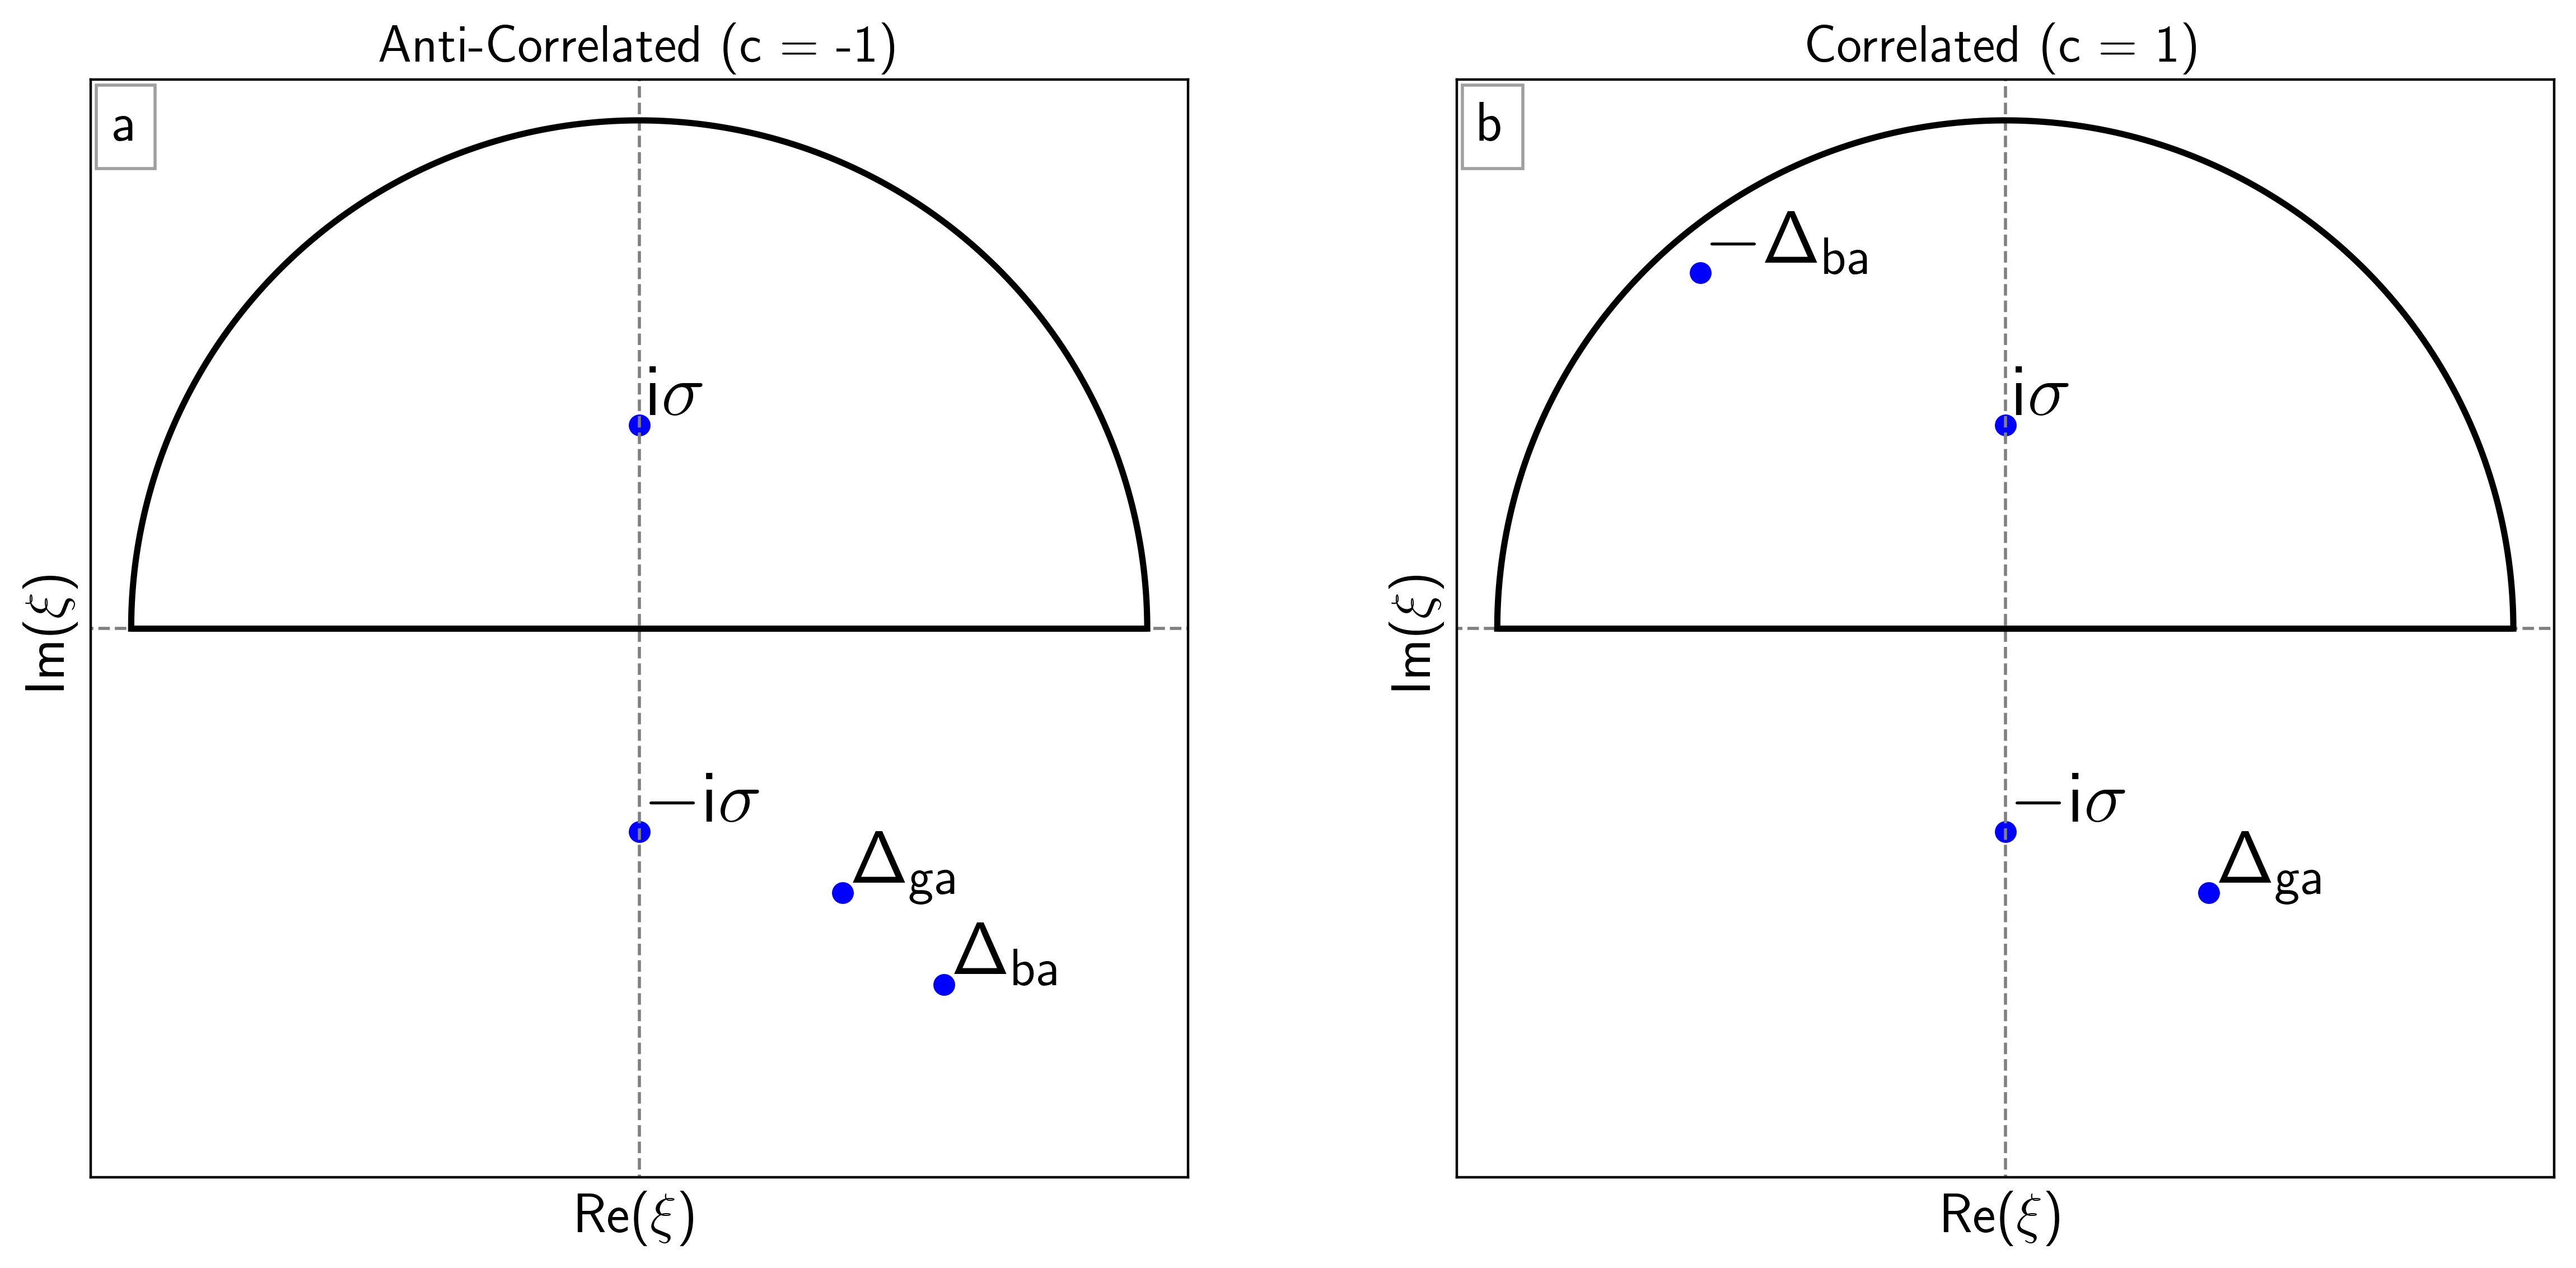
\includegraphics[width=3.375in]{main/corr_contour.png}
	\caption{Poles (black dots) and contour (blue line) used to evaluate \autoref{integraly} for (a) anti-correlated and (b) correlated modes.} 
	\label{fig:contours}
\end{figure}

\subsubsection{Anti-correlated Modes}
For anti-correlated modes, the poles are situated in the complex plane as shown in \autoref{fig:contours}a.
Since \autoref{integraly} is evaluated along the real axis, one can choose to evaluate the contour in the upper or lower half of the complex plane.
Since evaluating the residues in the upper or lower half of the complex plane yields the same result for \autoref{integraly}, we choose the contour which wraps around the least number of poles.

It is clear for c = -1 that there are four poles: $\pm i \sigma, \Delta_{ga}(0), \Delta_{ba}(0)$. 
Following \autoref{fig:contours}, the contour that wraps the upper half of the complex plane has only one pole, $i \sigma$; as such, we choose to evaluate \autoref{integraly} in the upper half of the complex plane for the case of anti-correlated modes through the residue theorem as
	\begin{equation}
		\begin{split}
			\rho_{ba} = \int_{-\infty}^\infty \mathrm{d}\xi P(\xi) \rho_{ba}(\xi) &= 2\pi i \sum_k \lim_{\xi \rightarrow \xi_k} P(\xi) \rho_{ba}(\xi) (\xi - \xi_k)\\
			&= 2\pi i \frac{\eta \sigma}{\pi} \lim_{\xi \rightarrow i\sigma} \frac{1}{(\xi + i\sigma)(\xi - i\sigma)} \frac{1}{\Delta_{ga}(0) - \xi} \frac{1}{\Delta_{ba}(0) - \xi} (\xi - i \sigma)\\
			&= 2 \eta \sigma i \lim_{\xi \rightarrow i\sigma} \frac{1}{\xi + i\sigma} \frac{1}{\Delta_{ga}(0) - \xi} \frac{1}{\Delta_{ba}(0) - \xi}\\
			&= 2\eta \sigma i \frac{1}{2i\sigma} \frac{1}{\Delta_{ga}(0) - i\sigma} \frac{1}{\Delta_{ba}(0) - i\sigma}\\
			&= \frac{\eta}{\Delta_{ga}(i\sigma)\Delta_{ba}(i \sigma)}\\
		\end{split}
	\end{equation}


In words, we see the inhomogeneous envelope width $\sigma$ is added to the linewidth of each resonance (e.g., $\Gamma_{ag} \rightarrow \Gamma_{ag} + \sigma$).
Therefore, pathway I-a cannot linenarrow anti-correlated modes. 
\subsubsection{Correlated Modes}
For correlated modes, the poles are situated in the complex plane as shown in \autoref{fig:contours}.
It is clear that no matter which contour is chosen, there is a contribution to the final integral from either $\Delta_{ba}(0)$ or $\Delta_{ga}(0)$. 
For the below calculation, we choose to evaluate along the contour in the bottom half of the complex plane, i.e., the poles ($\xi_k$) are $-i\sigma, \Delta_{ga}$.
We stress that since the integral is evaluated over $\mathbb{R}$ and there are no degenerate poles, the results below can be obtained by evaluating the contour which wraps around the poles $i\sigma, \Delta_{ba}$ using the Residue theorem as 

	\begin{equation}
		\begin{split}
			\int_{-\infty}^\infty \mathrm{d}\xi P(\xi) \rho_{ba}(\xi) &= 2\pi i \sum_k \lim_{\xi \rightarrow \xi_k} P(\xi) \rho_{ba}(\xi) (\xi - \xi_k)\\
			&= 2\pi i \frac{\eta \sigma}{\pi} ( \lim_{\xi \rightarrow -i\sigma} \frac{1}{(\xi + i\sigma)(\xi - i\sigma)} \frac{1}{\Delta_{ga}(0) - \xi} \frac{1}{\Delta_{ba}(0) - \xi} (\xi + i \sigma) \\ &+
			\lim_{\xi \rightarrow \Delta_{ga}(0)} \frac{1}{(\xi + i\sigma)(\xi - i\sigma)} \frac{1}{\Delta_{ga}(0) - \xi} \frac{1}{\Delta_{ba}(0) - \xi} (\xi - \Delta_{ga}))\\
%			&= 2 \eta i \sigma (\frac{1}{2 i \sigma} \frac{1}{-i \sigma - \Delta_{ga}(0)} \frac{1}{\Delta_{ba}(0) - i\sigma} ) - 2 \eta i \sigma (\frac{1}{\sigma^2 + (\Delta_{ga} (0))^2} \frac{1}{\Delta_{ga}(0) + \Delta_{ba}(0)} )\\
			&= -\frac{\eta}{\Delta_{ga}(0) + i \sigma} (\frac{1}{\Delta_{ba}(0) - i \sigma} + \frac{2i\sigma}{(\Delta_{ga}(0) - i \sigma)(\Delta_{ga}(0) + \Delta_{ba}(0))})\\
		\end{split}
	\end{equation}
The final line of the above equation shows the presence of a new term, $\frac{2i\sigma}{\Delta_{ga}(0) + \Delta_{ba}(0)}$. 
This term is amplified by the width of the inhomogeneous envelope ($\sigma$) and has a linewidth $\Gamma_{ba} + \Gamma_{ga}$, which linenarrows the transition. 
Results for the other pathways follow the same technique.
\end{widetext}
%Generally, when starting from the ground state, non-parametric spectroscopies line-narrow correlated modes, and parametric spectroscopies line-narrow anti-correlated modes. \cite{Dick83_1, RN425}


\section{References}
% Create the reference section using BibTeX:
\bibliography{library.bib}

\end{document}
%
% ****** End of file apstemplate.tex ******

